\subsection{Vliegstrategie}
\noindent {\em Auteur: Laura Vranken}
\\\\
\noindent
Vliegen rond een polyhedron om deze te kunnen scannen, vereist een zekere strategie. Ten eerste moet het mogelijk zijn om alle vlakken van het object te bekijken. Vervolgens moet bepaald worden wanneer de drone de volledige polyhedron heeft gezien en kan stoppen met deze te scannen. Ten slotte moet hij verschillende polyhedra van elkaar kunnen onderscheiden.
\\
Door een tekort aan tijd en onverwachte vertragingen is het laatste punt niet uitgewerkt. Het vervolg van deze paragraaf gaat dus enkel verder in op het scannen van één polyhedron.
Hoewel deze strategie volledig uitgewerkt is, wordt tijdens de demo gevlogen op basis van een op voorhand ingestelde baan van het Testbed. Dit doordat het huidige vliegen van de Autopilot nog niet nauwkeurig genoeg is om gecontroleerd rond een polyhedron te vliegen.
\\\\
Er wordt gestart vanuit het beginbeeld met de polyhedron recht voor de drone. Elke zichtbare driehoek wordt gesplitst in zijn drie zijdes en deze worden in een lijst bijgehouden. Aangrenzende driehoeken delen altijd eenzelfde zijde. Wanneer dus beide driehoeken van een zijde herkend zijn, kan deze zijde uit de lijst verwijderd worden en als gezien geklasseerd worden. Als deze lijst leeg is, kan vervolgens besloten worden dat beide driehoeken van elke zijde gescand zijn en dat de polyhedron volledig afgewerkt is.
\\\\
Om volledig rond de polyhedron te kunnen vliegen, wordt telkens bepaald uit de lijst welke zijde nog een driehoek mist. De voorkeur gaat uit naar een zijde die het dichtst in de buurt van de drone ligt en zal dus degene zijn die het laatst is toegevoegd. Het doel is te vliegen naar een bepaalde positie waaruit die zijde en zijn aanliggende driehoeken kunnen waargenomen worden. Die positie wordt door het volgende algoritme bepaald.
\\
Eerst wordt een rechte getrokken tussen de drone en het zwaartepunt van de gekende driehoek. Vervolgens wordt er op die rechte een punt gekozen dat iets verder ligt dan de driehoek. Het is een schatting van het centrumpunt van de polyhedron. Vervolgens wordt een nieuwe rechte getrokken vanuit dit centrumpunt door het middelpunt van de te bekijken zijde. Hierop wordt opnieuw een punt gedefinieerd, dit keer op een afstand van 1 meter van de polyhedron. Dat punt is de nieuwe volgende positie naar waar gevlogen moet worden. Het algoritme wordt ge\"illustreerd in Figuur \ref{fig:ScanFly}.
\\
\begin{figure}[H]
\centering
	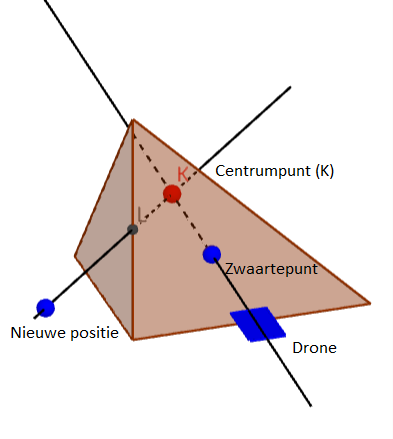
\includegraphics[width=0.4\textwidth]{Scannen/FigStrategieScan.png}
	\caption{Bepalen van de nieuwe positie om de zijde en aanliggende driehoek te zien.}
    \label{fig:ScanFly}
\end{figure}